% This first statement determines the overall format of the document.
% There are a number of built in types e.g., article.  But many journals
% and conferences have their own documentclass definition.
% We will be using IEEETtran.  Note that, in order to use IEEEtran, you
% will need the IEEEtran.bst and IEEEtran.cls files in the same folder as
% your main file.

% The % character is the start of a comment.
% If you want to have Latex print % you need to use \ before the % symbol.


\documentclass{IEEEtran}
%\documentclass{article}
\usepackage{wrapfig}
\usepackage{graphicx}
\usepackage{float}
\usepackage[export]{adjustbox}
\usepackage{fixltx2e}
\usepackage{authblk}

%\usepackage{mdframed}

\title{Automated Drug Repurposing: Evolving Drug Discovery via Faster Biomedical Data Extraction}
\author{Dylan Lehrer}
\date{}

\begin{document}
	\bibliographystyle{plain}
	\maketitle
	\pagestyle{plain}
	
	\begin{abstract}
	Low success rates and high costs plague modern drug development, which generally costs \$500 million to \$2 billion, spans approximately 12 years, and is often considered inefficient and risky~\cite{kaitin}.  Computer-aided drug discovery has been exhaustively explored for more than three decades, but recent breakthroughs have invigorated the industry and medicine's future.  More efficient drug discovery processes stem from technological growth and biomedical database expansion, while drug repurposing, despite inefficient manual data extraction~\cite{zhang15},~\cite{zhang16}, has emerged as a cost-effective alternative to old ways.  
	
	Like drug discovery and other inefficient processes, drug repurposing efforts can be enhanced through automation. Identifying valuable automated drug repurposing tools, we have developed an automated drug repurposing framework.  Our working prototype takes individual disease name input, utilizes interconnected tools to extract and retrieve disease-related biomedical data, and outputs individually weighted pre-approved drugs for potential disease-specific treatment.  Compared to manual drug repurposing efforts~\cite{zhang16}, our automated prototype identifies 70 of 92 (76\%) recommended drugs for Alzheimer's disease, but 14,852 drugs are suggested.  Reducing unimportant automated drug suggestions through more drug data integration and comprehensive filtering, this model could replicate manual studies while saving time and money.
	\end{abstract}
	
	\tableofcontents
	\listoffigures
	\listoftables
	
	\section{Introduction}
		Investing time and money does not guarantee drug development success.  New drug development\textemdash from research labs to patients\textemdash costs approximately \$500 million to \$2 billion\textemdash in addition to about 12 years necessary for drug approval~\cite{cbra},~\cite{boguski}.  Only 2\% of drugs in pre-clinical testing are eventually approved for human administration~\cite{cbra}.  Due to low success rates and large amounts of time and money involved in creating new and approved drugs, the drug development process is often considered inefficient and risky~\cite{kaitin}.  
		
		Alternative drug discovery processes had been nearly exhausted, but recent in silico (computer-aided) drug discovery breakthroughs have invigorated the industry and medicine's future.  With technology progression and biomedical database expansion, efforts to employ more efficient drug discovery processes have emerged and become more practical. Drug repurposing, though inefficiently executed via manual data extraction~\cite{zhang15},~\cite{zhang16}, has arisen in recent years as a promising, cost-effective alternative to traditional drug development. As the world's inefficient processes continue to be enhanced by automation, and given patterns of increasing technological growth and data availability, we envision a similar, automated future for drug repurposing. By identifying and using  new technological tools and resources, we have created an automated drug repurposing framework and working prototype that could rival manual drug repurposing methods and lead to more efficient drug discovery. 
	
		\section{Pre-Technological Drug Discovery}
		\subsection{Early Medicine}
		Early civilizations used different types of treatments as physical, religious, and/or spiritual healing remedies.  Without advanced chemical knowledge and technological resources, these methods most likely consisted of extensive trial and error periods, where humans and animals were administered treatments (``drugs") in efforts to combat illnesses.  If conditions improved after receiving treatment, one could assume the respective remedy had healing potential for the illness it was tested against.  With more knowledge and shared experiences, effects of ingesting certain folk medicines could be hypothesized, but trial and error methods did not produce safe and efficient results in early drug discovery efforts \cite{ng}. 
		\subsection{Synthetic Drug Products}
		Drugs can now be produced from synthetically created chemical compounds in addition to natural products.  These pharmaceutical compounds are manufactured through complex chemical syntheses\textemdash sequences of chemical reactions resulting in desired chemical products.  Beginning in the early 1900s, with a more complete knowledge of chemistry and disease, chemical methods enabled development of synthetic drug compounds and the pharmaceutical industry, where many early drugs provided therapeutic relief from disease symptoms \cite{ng}.
		\subsection{Standardized Drug Development} \label{standardized}
		Development of new and improved chemical methods and drug design strategies led to more structured drug discovery.  Today's drug discovery process consists of a methodical and multi-faceted approach of ``seven [key] steps: disease selection, target hypothesis, lead compound identification (screening), lead optimization, pre-clinical trial, clinical trial, and pharmacogenomics optimization" \cite{xu}. 
		\begin{figure*}
			\centering
			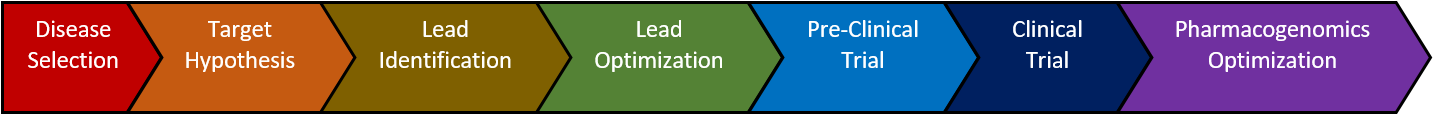
\includegraphics[width=\textwidth, scale=0.5]{Fig1}
			\caption{\footnotesize Seven traditional drug development steps in the order they most often occur (beginning with disease selection and ending with pharmacogenomics optimization).}
			\label{fig1}
		\end{figure*}
		\begin{enumerate}
			\item \textbf{Disease Selection:} In the disease selection phase, information must be gathered on the illness/disease in question, and extensive research is usually performed to better understand its cause(s) and potential treatment method(s). 
			\item \textbf{Target Hypothesis:} Using gathered knowledge on single diseases, scientists can hypothesize specific proteins or bodily pathways that might lead to undesirable disease states.  These respective proteins and/or pathways might need to be inhibited or activated to therapeutically improve disease effects.  Drug targets (usually proteins) are molecules within living organisms that drugs can bind, and target hypotheses should be validated before moving on to the next step \cite{xu}.
			\item \textbf{Lead Identification:} After the target is validated, fragments, compounds, and/or other biological materials in compiled libraries are screened directly against the drug target for activity, identifying whether or not the compound successfully interacted with the target site, resulting in a ``hit."  These libraries generally provide access to several thousand unique compounds\textemdash the Stanford High-Throughput Bioscience Center (HTBC) compound library currently contains over 130,000 diverse compounds \cite{stan}.  Nowadays, compounds can be quickly screened using advanced robotics, data processing, and software.  Different screening approaches look for various features to define successful activity effects at the target site.  These screening approaches include:
			\begin{itemize}
				\item \textit{High throughput screening (HTS)}: every compound in the library is screened.
				\item \textit{Focused (knowledge-based) screening}: only the most promising molecules, based on pre-existing knowledge, are screened.
				\item \textit{Fragment screening}: only low molecular weight compounds are screened.
				\item \textit{Physiological screening}: live bodily tissues, rather than individual molecular components, are screened.
			\end{itemize} 
			Screening approaches allow for the identification of leads, molecules that positively interact with the drug target.  There has been significant interest in exploring the lead discovery phase for pharmaceutical purposes in recent years \cite{hughes}.
			\item \textbf{Lead Optimization:} Identified lead compounds are active at the drug target site and may be therapeutically useful, but can still have suboptimal structure.  The structure and properties of identified lead compounds can be optimized to better fit the target site in the lead optimization phase.
			\item \textbf{Pre-Clinical Trial:} After optimizing lead compounds, potential drugs must be tested on animal models in the lab.  These trials reveal safeness of testing drugs on human patients. 
			\item \textbf{Clinical Trial and Pharmacogenomics Optimization:} Once deemed safe for human ingestion, healthy volunteers receive candidate drugs in clinical settings, and researchers note related drug effects.  Pharmacogenomics, ``the study of how genes affect [an individual's] response to drugs," strives for maximal safety and effectiveness in these clinical trials \cite{nih}, \cite{surend}.   Pharmacogenomics optimization applies the study of pharmacogenomics to determine who specific drugs will best serve, and at what dose medications should be administered to different types of patients \cite{surend}. This optimization step is important because drugs will not work the same way for everyone, and genetic differences could cause certain medications to have no effect or negative effects amongst particular individuals at given doses.   Drugs that persistently meet expectations in clinical trials are administered to larger groups of patients in different locations.  With a sufficiently large sample size and an appropriately described treatment protocol, drugs can eventually be reviewed and approved for their effects and overall safety by the U.S. Food and Drug Administration (FDA), marking the conclusion of the lengthy and complex drug development process \cite{hughes}, \cite{nih}.
		\end{enumerate}
		\subsection{Drug Repurposing} \label{drugrepurp}
		Also known as drug repositioning, drug repurposing involves applying already marketed and approved drugs to new indications, as displayed in Figure~\ref{repurp}. Drug repurposing is faster and cheaper than traditional drug discovery, because it bypasses the lengthy timeframe needed to develop and approve new drugs.  Since many readily available drugs have already been tested and deemed safe for human ingestion, there has been a recent focus on repurposing marketed drugs for new indications in the field of drug discovery~\cite{boguski}
		
		\begin{figure}[h]
			\centering
			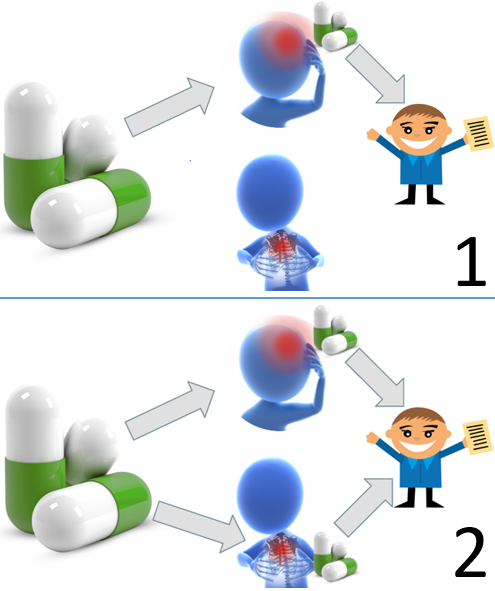
\includegraphics[width=\linewidth]{repurp}
			\caption{\footnotesize Simplified representation of the drug repurposing process\textemdash applying a pre-approved drug to therapeutically treat a new indication. The fictional green and white pill pictured, first approved to treat head pain, is repurposed to treat a disease causing chest problems.}
			\label{repurp}
		\end{figure} 
	
		\section{In Silico Drug Discovery}
		\subsection{Shifting Towards Technology}
		Historically, drug discovery has been limited by drug development and testing costs. Since the 1980s, however, computers have accelerated drug discovery steps through modeling and simulation processes~\cite{sliwo}.
		
		Beginning in 1980, HTS enabled computerized screening and the ability to screen hundreds of thousands of compounds per drug target per year \cite{gall}, \cite{hecht}.  This technological improvement made chemists unable to make enough new compounds to meet the demands of biologists.  This gap was slightly narrowed through combinatorial chemistry (CC), which allowed chemists to produce many synthetic compounds with large structure libraries. These quickly created chemical compounds could have significantly accelerated the drug discovery process, but many of the millions of compounds made by CC technologies were not potential drug candidates; the compound libraries needed more chemical diversity.
		
		In order to optimize CC technology use, computational approaches created compound libraries with more drug candidates and greater chemical diversity.  Approaches such as ``structural descriptor computations, structural similarity algorithms, classification algorithms, diversified compound selections, and library enumerations" were developed in the 1990s~\cite{xu}.  These approaches formed more chemically diverse libraries, which generated more hits.  However, this didn't guarantee new drugs being developed from these chemical starting points~\cite{xu}.  Many compounds created in chemically diverse libraries were not drug-like in their properties and never developed into drugs.  In the early 2000s,  new technologies began recognizing drug-like compounds in chemically diverse libraries of compounds for subsequent screening against biological drug targets, solving this problem ~\cite{begam},~\cite{brown},~\cite{xu}.
		
		\subsection{Data-Driven Drug Discovery}
		Availability of chemical and biological data has driven aforementioned computer-based methods.  Chemical structures are now represented within chemical datasets by linear notations\textemdash such as the Wiswesser Line Notation (WLN), Simplified Molecular Line Entry System (SMILES), and International Chemical Identifier (InChI)\textemdash which machines can read, write and interpret~\cite{xu}.
		
		\begin{table}[H]
			\begin{center}
				\begin{tabular}{|c|c|c|c|} \hline
					\textbf{Formula} & \textbf{SMILES} & \textbf{InChI} \\ \hline
					$C_2H_6$ & CC & InChI=1S/C2H6/c1-2/h1-2H3   \\ \hline
					$CO_2$ & O=C=O & InChI=1S/CO2/c2-1-3  \\ \hline
					$HCN$ & C\#N & InChI=1S/CHN/c1-2/h1H  \\ \hline
					$C_6H_6$ & c1ccccc1 & InChI=1S/C6H6/c1-2-4-6-5-3-1/h1-6H \\\hline
				\end{tabular}
				\caption{\footnotesize SMILES and InChI notations for ethane ($C_2H_6$), carbon dioxide ($CO_2$), hydrogen cyanide ($HCN$), and benzene ($C_6H_6$).  Unique notations are produced for different chemical structures.}
			\end{center}
		\end{table}
		The WLN was considered the best linear notation from the late 1960s to 1980s, but SMILES and InChI are more widely recognized and accepted by chemical databases today for their simplified form and the breadth of chemical properties they can account for~\cite{xu}. 
		
		Chemical and biological datasets are often very large (millions of records) and quickly growing, so they can be more cost- and time-effectively analyzed using computer algorithms than humans.  Additionally, chemical and lab material costs make lab-based chemical experimentation very expensive.  To reduce costs, chemical and biological data drive current drug discovery, with the goal of discovering new knowledge from existing data (data mining).  
		
		Larger data supplies have driven approaches that collect, organize, and analyze new chemical and biological information before applying it to drug discovery processes~\cite{begam}.  Most drug discovery research computational methods involve cheminformatics and/or bioinformatics\textemdash relatively new and emerging disciplines that process chemical and biological data, respectively, using computers.  Cheminformatics and bioinformatics analysis methods can reduce drug development step costs, making drug development faster, cheaper, and more efficient~\cite{begam},~\cite{brown},~\cite{xu}.  Major cheminformatics and bioinformatics applications in drug discovery include data mining to predict drug targets~\cite{elshi}, compound-target interactions~\cite{keum}, drug side effects~\cite{atias}, and drug label changes~\cite{guru}.
		
		\subsection{Systems-Oriented Drug Repurposing}
		Many diseases are well understood, but occasional challenges arise in translating physiological and molecular understanding into disease-combatting drugs and/or remedies.  Systems-oriented drug discovery approaches construct comprehensive molecular biomolecular system models.  This differs from more traditional drug discovery approaches, where many believed single drugs could only correspond to one target.  Systems-oriented models allow many thousands of different molecular entities to be simultaneously studied as parts of more expansive biomolecular systems.  Systems-oriented drug discovery approaches can be applied to drug repurposing, target discovery, and drug toxicity analysis~\cite{dud}.
		
		\subsection{Literature Mining}
		
		In 2011, with a quickly growing database of biochemical information in PubMed, researchers turned to text mining (data mining of text) to create linked networks, bringing together articles that contained similar concepts or arguments that aren't necessarily mentioned together in one single article.  This text mining process is known as literature-based discovery (LBD).  LBD in biomedical literature is useful for finding new uses for existing drugs (i.e., drug repurposing~\cite{andronis}.  One very recent area of growth at the intersection of literature mining and drug repurposing is drug repurposing based on `omics' data mining~\cite{zhang15},~\cite{zhang16}.  
	
	\subsection{`Omics' Data Mining} \label{omics}
	The evolving method of drug repurposing based on omics data mining was first publicized in a 2015 study that extracted frequently referenced data on genes, proteins, and metabolites from diabetes-related scientific literature~\cite{zhang15}.  Referred to as omics data because of the -omics suffix in genomics, proteomics, and metabolomics, three biological fields of study, manually extracted data was used to find diabetes-related proteins and connected to several databases to conclude top potential pre-approved drugs for therapeutic treatment.  Drug filtering methods pinpointed nine drugs as potential diabetes treatments.  Six of the nine drugs were repurposed to treat type 1 or type 2 diabetes.  The study suggested similar omics data mining approaches could be used to therapeutically treat other disorders, such as Alzheimer's disease (AD), through drug repurposing~\cite{zhang15}.  
	
	In 2016, Zhang et al.~\cite{zhang16} explored the use of drug repurposing based on omics data mining for the treatment of AD.  This study identified 524 AD-related proteins, 8 possible protein targets for anti-AD drug development, and 18 protein targets linked to 92 existing drugs for potential AD treatment repurposing~\cite{zhang16}.  Again, this study's data extraction was manually performed.  Using omics data mining in drug repurposing efforts has produced promising results that suggest these methods could be valuable in discovering new treatments for more diseases, but we believe automating this process will lead to less time wasted and more medical discoveries.
	
	\section{Future Drug Discovery: Automative Trends}
	\subsection{Future Drug Repurposing}
	Like most inefficient processes and drug discovery, drug repurposing efforts can be revitalized via automation. Bypassing lengthy drug approval protocol, drug repurposing seems well-suited to transition towards automated methods. After identifying potential repurposed drugs through automation, closer testing could ensure safe and viable drug ingestion under new, specific indications.  Automation within the next five years could elicit drug repurposing success by providing direction and narrowing results to more manageable testing sets, saving additional time and money. However, an ideal automation system would more accurately identify repurposable drugs and eliminate clinical testing necessities. 
	
	\subsection{Technological Growth and Biomedical Data Abundance} \label{tgbd}
	The past two decades' internet growth has revolutionized data sharing\textemdash generating more chemical and biological data~\cite{boguski}.  Sharing-based biomedical research communities regularly contribute experimental and open-access data to large databases managed by institutions such as the National Institutes of Health (NIH) and the European Molecular Biology Laboratory (EMBL)~\cite{youtube}. With recent molecular technology advances, biological and chemical data supplies have exponentially increased~\cite{cook}.
		
		PubMed, one of several free search services developed by the National Center for Biotechnology Information (NCBI), provides access to over 26 million biomedical literature abstracts and citations~\cite{pubmed}. PubMed has benefited from data sharing tendencies.  Since 2011, the database has grown at a rate of over 850,000 abstracts per year~\cite{andronis}, and steadily increased at a rate of over 1.1 million abstracts per year from 2004 to 2017~\cite{pubmedstats}, as seen in Figure~\ref{pubmed}.
		\begin{figure}[h]
			\centering
			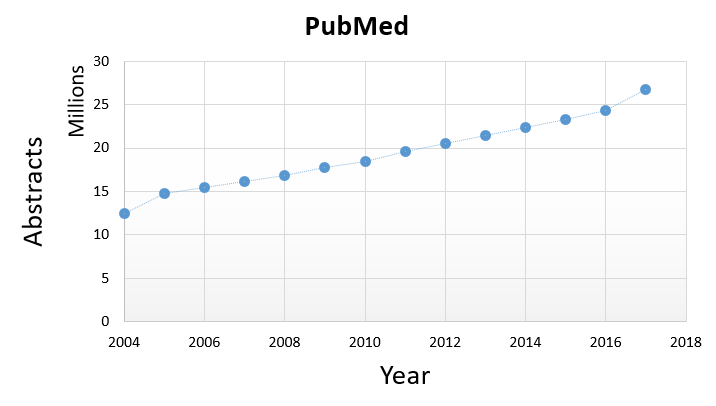
\includegraphics[width=\linewidth]{pubmed}
			\caption{\footnotesize A plot of PubMed abstracts over time, showing the growing amount of biomedical data available for processing. PubMed now contains over 26 million abstracts and has steadily increased at a rate of over 1.1 million abstracts per year from 2004 to 2017~\cite{pubmedstats}.}
			\label{pubmed}
		\end{figure}
		
		Due to PubMed's vast scientific literature collection and search filter variety, it can be used to find publications containing relevant information between multiple keywords, and the results of a simple multi-parameter search can clue into relative topic similarity.
		
		Other large databases managed by institutions such as the National Institutes of Health (NIH) and the European Molecular Biology Laboratory (EMBL) offer similar features to PubMed and continue to grow.  Specialized data resources provide protein, gene, disease, drug, and/or metabolic data.  For example, the Universal Protein Resource Knowledgebase (UniProtKB)/Swiss-Prot database, one of the NCBI Protein database's seven constituents~\cite{oxford}, contains information on over 20,000 human proteins~\cite{uniprot},~\cite{RN54}.  
		
		Therapeutic Target Database (TTD) and DrugBank, useful drug repurposing databases, both curate information on human protein targets and drug projects (drugs at any approval stage) acting upon them.  ``Drugs generally exert their therapeutic effect by binding to a particular protein or nucleic acid target"~\cite{ttd02},~\cite{drugbank06}, and each protein target in these databases is linked to one or more drugs. TTD (Figures~\ref{ttdprot} and~\ref{ttddrug}) and DrugBank (Figures~\ref{dbprot} and~\ref{dbdrug}), both updated regularly, have followed similar patterns of growth.  Compared to TTD's 433 non-redundant protein targets and 809 drug projects in 2002~\cite{ttd02}, it currently contains data on 2,589 protein targets and 31,614 drug projects~\cite{ttd16}. 
		
				\begin{figure}[h]
					\centering
					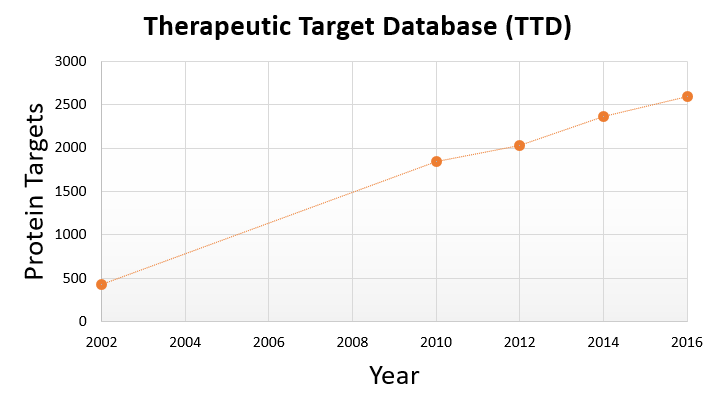
\includegraphics[width=\linewidth]{ttdprot}
					\caption{\footnotesize A plot of unique TTD protein targets over time, increasing in every statistical report from 2002 to 2016~\cite{ttd02},~\cite{ttd14},~\cite{ttd16},~\cite{ttd10},~\cite{ttd12}.}
					\label{ttdprot}
				\end{figure} 
				\begin{figure}[h]
					\centering
					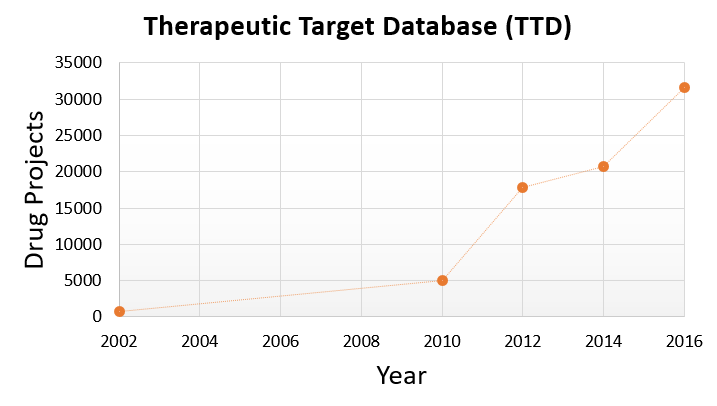
\includegraphics[width=\linewidth]{ttddrug}
					\caption{\footnotesize A plot of unique TTD drug projects over time, increasing in every report from 2002 to 2016~\cite{ttd02},~\cite{ttd14},~\cite{ttd16},~\cite{ttd10},~\cite{ttd12}.}
					\label{ttddrug}
				\end{figure}
		DrugBank, created in 2006 with 3,909 drug projects and 2,133 protein targets~\cite{drugbank08},~\cite{drugbank06}, now contains data on 8,261 drug projects and 4,338 protein targets~\cite{drugbank14}.  Additionally, DrugBank has added more detailed drug data, such as drug metabolism and pathway information~\cite{drugbank14}.
		
		\begin{figure}[h]
			\centering
			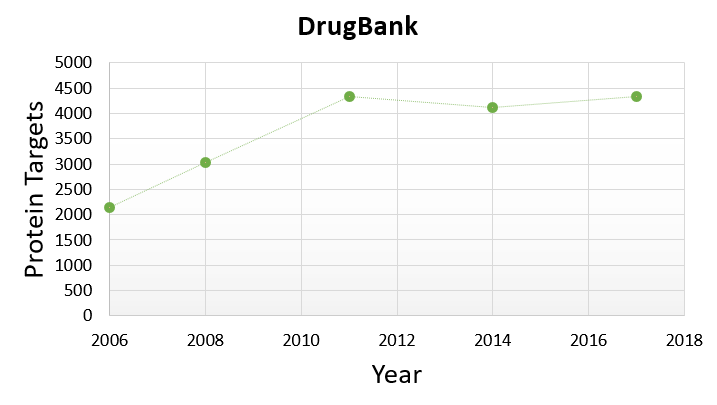
\includegraphics[width=\linewidth]{dbprot}
			\caption{\footnotesize A plot of unique DrugBank protein targets over time, increasing in all but one report from 2006 to 2017~\cite{drugbank14},~\cite{drugbank08},~\cite{drugbank06}.}
			\label{dbprot}
		\end{figure}
		\begin{figure}[h]
			\centering
			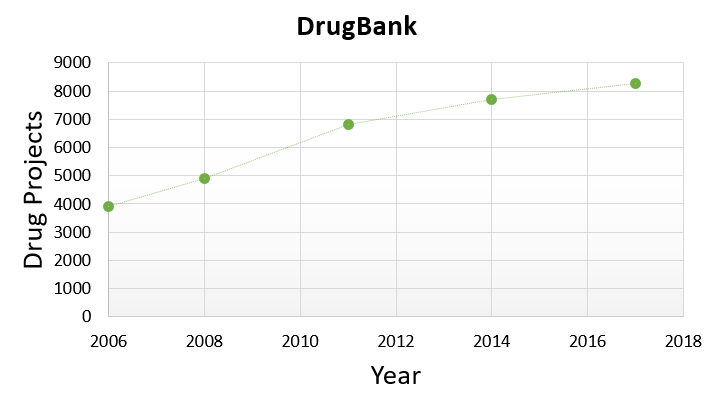
\includegraphics[width=\linewidth]{dbdrug}
			\caption{\footnotesize A plot of unique DrugBank drug projects over time, increasing in every report from 2006 to 2017~\cite{drugbank14},~\cite{drugbank08},~\cite{drugbank06}.}
			\label{dbdrug}
		\end{figure}
		
		
		As seen in Figures~\ref{ttdprot},~\ref{ttddrug},~\ref{dbprot}, and~\ref{dbdrug}, TTD and DrugBank have grown consistently over time, storing more valuable data and becoming more useful to drug discovery researchers. TTD and DrugBank will likely continue to grow for several years; however, they are meritable in their current states, and only a small sampling of many available biomedical datasets. In the future, new, better, and more comprehensive databases could arise, further improving automated drug discovery resources. 
		
		The growth of useful data fuels automation.  As valuable biomedical data sources continue to fill with accurate information, more relevant disease, protein, gene, and drug connections can be made.  Similar to students learning more by consulting larger book selections, automated drug discovery programs will likely learn better from, and operate more reliably with, increasingly comprehensive datasets like PubMed, TTD, and DrugBank.
	
	\subsection{Rare Diseases}
	
	 States, diseases that affect less than 200,000 individuals are considered ``rare"~\cite{raredis}. Over 6,500 diseases are identified as rare diseases, which collectively affect more than 30 million\textemdash or approximately 1 in 10 (Figure~\ref{rd2})\textemdash Americans worldwide~\cite{raredis}. 
	
	\begin{figure}[h]
		\centering
		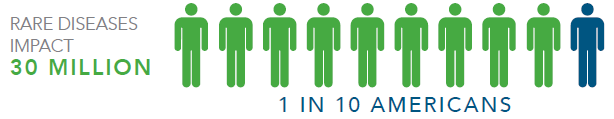
\includegraphics[width=\linewidth]{rd2}
		\caption{\footnotesize Visual depiction of United States rare disease prevalence. Approximately 10\% of Americans have been diagnosed with at least one of over 6,500 rare diseases.}
		\label{rd2}
	\end{figure} 
	
	The pursuit of therapeutic measures for rare diseases is less attractive to the biopharmaceutical industry because of limited market appeal and earning potential relative to more common diseases affecting more people and needing more frequent treatment. Approximately 90\% of all rare diseases do not have any specific treatment. Many believe new medicines must be created to treat the majority of rare diseases, but treatments for rare diseases could be found through drug repurposing. Over 80\% of rare diseases are considered genetic in origin~\cite{raredis}. Sometimes, rare-disease causing genes share biological processes or pathways with common disease-associated genes, and resulting connections could suggest effective treatment discoveries through linked data.  
	
	Given the sheer number of rare diseases, automation could make drug discovery faster and more viable for less profitable, small market diseases.  However, some rare diseases lack adequate data. More research is dedicated to diseases that affect larger contingents of people. This research is generally more relevant and profitable to the biomedical community.  Correspondingly, PubMed searches for rare diseases typically return fewer results than high-profile diseases like diabetes and AD.  Inadequate disease-specific data and pre-existing knowledge limits automated method effectiveness for some rare diseases, however, with more devotion to studying rare diseases, potential for automated therapeutic treatment discovery still exists.
	
	
	\section{Automated Drug Repurposing Tools}
	\subsection{Therapeutic Target Database}
	Used by Zhang et al. in manual drug repurposing efforts for diabetes~\cite{zhang15} and AD~\cite{zhang16}, the TTD provides interconnected human protein target drug project data\textemdash as briefly discussed in Section~\ref{tgbd}.
	
	Seen in Table~\ref{ttduniprotall}, a sampling from one of three useful datasets produced from TTD information, proteins showing therapeutic target potential are assigned locally unique TTD Target IDs in addition to more widely recognized Universal Protein Resource (UniProt) IDs~\cite{ttd10}. Table~\ref{ttduniprotall} also shows established links between TTD Target IDs, protein target names, and the latest level of success acting on that specific protein target (i.e., which testing stage: successful, clinical trial, research, or discontinued).
	\begin{table}[h]
		\centering
		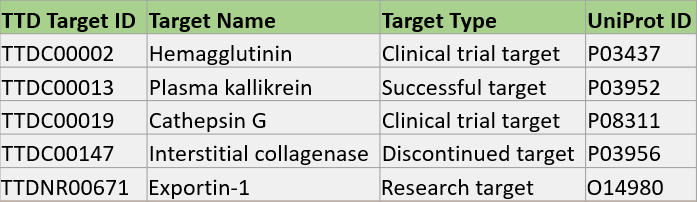
\includegraphics[width=\linewidth]{ttduniprotall}
		\caption{\footnotesize Five records from a TTD dataset including proteins that exhibit therapeutic target potential, regardless of their testing stage.  Local TTD Target IDs are linked to protein target names, protein target testing stages, and globally recognized UniProt IDs.}
		\label{ttduniprotall}
	\end{table} 

	
	Another frequently used TTD dataset can be seen in Table~\ref{ttdtargetdisease}, where protein targets, and their respective TTD Target IDs, are linked to one or more indications (diseases) that drugs have attempted to treat by binding those respective proteins.  Indications correspond with International Classification of Diseases (ICD) codes that enable less ambiguous identification and information retrieval between datasets.
		\begin{table}[h]
			\centering
			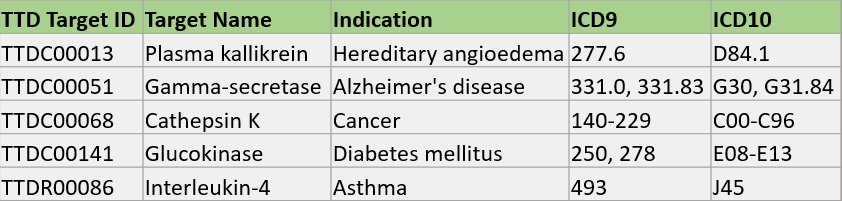
\includegraphics[width=\linewidth]{ttdtargetdisease}
			\caption{\footnotesize Five records from a TTD dataset mapping protein targets (by TTD Target IDs and Target Names) to indications and their globally recognized ICD codes. Individual protein targets can be linked to more than one indication.}
			\label{ttdtargetdisease}
		\end{table}

	Similar to the target-disease relationships shown in Table~\ref{ttdtargetdisease}, Table~\ref{ttddrugdisease} illustrates drug-disease relationship information available in another TTD dataset.  Drug projects (drugs at any approval stage) are assigned unique TTD Drug IDs, which are linked to individual drug names, drug indications, and the ICD codes of these indications.  
	\begin{table}[h]
		\centering
		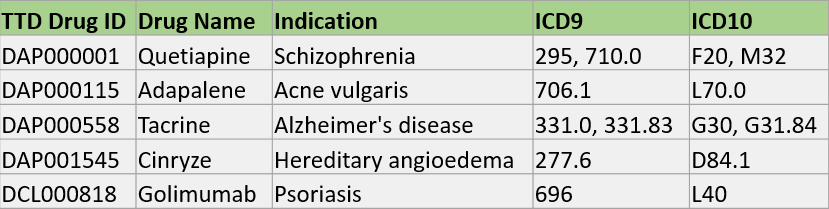
\includegraphics[width=\linewidth]{ttddrugdisease}
		\caption{\footnotesize Five records from a TTD dataset mapping drug projects (by TTD Drug IDs and Drug Names) to indications and their globally recognized ICD codes.  Drug projects will always map to one indication.}
		\label{ttddrugdisease}
	\end{table}	
	
	The datasets shown in Tables~\ref{ttduniprotall},~\ref{ttdtargetdisease}, and~\ref{ttddrugdisease} all derive from the TTD, which is updated regularly and currently contains data on 2,589 protein targets (397 successful, 723 clinical trial, and 1,469 research) and 31,614 drug projects (2,071 approved, 9,528 clinical trial, and 17.803 experimental)~\cite{ttd16}.
	\subsection{PubMed}
	As mentioned in Section~\ref{tgbd}, PubMed contains a large and growing selection of searchable biomedical literature. One of PubMed's distinguishing features is its U.S. National Library of Medicine (NLM) Medical Subject Headings (MeSH) assigned to all articles~\cite{mesh15}.  Trained professionals manually index articles with MeSH terms according to standardized methods, which ensures accurate assignments to articles covering MeSH topics~\cite{mesh01}.  In 2016, over 80,000 MeSH terms mapped to 27,883 article descriptors after synonym consolidation~\cite{mesh15}.  Varied MeSH terms with synonymous aliases link articles to topics such as diseases and symptoms\textemdash improving PubMed's filtered search capabilities and reducing nomenclature ambiguity, a prominent text mining challenge~\cite{hsdn}.
	\subsection{Protein Database}
	The NCBI Protein database contains protein sequence information from databases such as the UniProtKB, Swiss-Prot, the Protein Information Resource (PIR), the Protein Research Foundation (PRF), the Protein Data Bank (PDB), GenBank, and RefSeq~\cite{oxford}.  Protein database search results include information on proteins related to provided keywords.  These searches can be filtered by organism and source database.  Using only the UniProtKB/Swiss-Prot source ensures all protein search results will include UniProt IDs.
	\subsection{Entrez Programming Utilities}
	The Entrez Programming Utilities (E-utilities) are a set of nine server-side programs (meaning they can be run through your own program and outside of the web browser)~\cite{eutilities}. An application programming interface (API), a set of rules, protocols, and tools for building software and applications~\cite{eutils}, E-utilities allows for more detailed search and retrieval from the NCBI's Entrez databases (including PubMed, Protein, and Gene).  The E-utilities use a fixed URL syntax that translates a standard set of input parameters into values necessary for various NCBI software components to search for and retrieve requested data.  Each E-utilities URL consists of three parts~\cite{eutils}:
	\begin{enumerate}
		\item \textbf{E-utilities server address:} Every URL begins with \textit{https://eutils.ncbi.nlm.nih.gov/entrez/eutils/}
		\item \textbf{Utility name:} The name of one of nine E-utilities\textemdash ESearch, ESummary, EFetch, EPost, ELink, EInfo, ESpell, ECitMatch, or EGQuery\textemdash that perform different functions, followed by the `.fcgi?' file extension.
		\item \textbf{Parameters:} The items\textemdash such as database name, search terms, and result format\textemdash passed to the utility tool that determine query output.
	\end{enumerate}
	
	Given this three part structure, E-utilities URL functions are often easily decipherable, as seen in the following separated URL: 
	\begin{enumerate}
		\item \textit{https://eutils.ncbi.nlm.nih.gov/entrez/eutils/}
		\item \textit{esearch.fcgi?}
		\item \textit{db=pubmed\&term=nature[journal]+AND+3D+printing}
	\end{enumerate}
	The three URL parts always appear in this order.  In all cases, the server address remains consistent, and in this specific example, the utility\textemdash which appears before the .fcgi? extension\textemdash is ESearch.  The two parameters in the URL, \textit{db} and \textit{term}, can be identified by trailing equal signs.  In this case, the \textit{db} parameter specifies the PubMed database, while \textit{term}, the text searched for, is ``nature" in the journal field and ``3D printing" in any field~\cite{eutils}.  E-utilities are used extensively in programs accessing Entrez databases, so understanding their basic structure is useful in harnessing their searching capabilities.    
	
	\subsection{Entrez Direct}
	Entrez Direct (EDirect) is a software suite that provides access to the NCBI's interconnected databases from the UNIX command line.  The EDirect package\textemdash created in 2013\textemdash consists of several UNIX shell scripts that can be called as functions to use E-utilities from the command line~\cite{edirect14},~\cite{edirect17}.  All EDirect files are downloadable through a File Transfer Protocol (FTP) command in the terminal.  After EDirect software installation, EDirect functions allow for database navigation, record retrieval, field extraction, and more.  Five key EDirect functions are summarized below~\cite{edirect17}.
	\begin{itemize}
		\item \textbf{esearch:} searches an Entrez database using provided terms in indexed fields.
		\item \textbf{elink:} looks for close inter- and intra-database relationships.
		\item \textbf{efilter:} filters previous query results.
		\item \textbf{efetch:} retrieves records in a specific format.
		\item \textbf{xtract:} extracts specified attributes by parsing and converting standardized XML results to a table of values.
	\end{itemize}
	
	These functions can be combined to produce detailed queries and specific search results.  Using EDirect commands, more precise queries can be made to Entrez databases, and any field referenced in database XML metadata (data that describes other data) can be accessed and extracted from the command line in a manner that best fits the user's purpose.
	\subsection{Human Symptoms-Disease Network}
	In 2014, Zhou et al.~\cite{hsdn} utilized PubMed's MeSH metadata and text mining techniques to publish the Human Symptoms-Disease Network (HSDN), a symptom-based disease network constructed via symptom-disease relationship extraction from 849,103 PubMed bibliographic records. The network contains 147,978 connections between 322 symptoms and 4,219 diseases~\cite{hsdn}.
	
	\begin{table}[h]
		\centering
		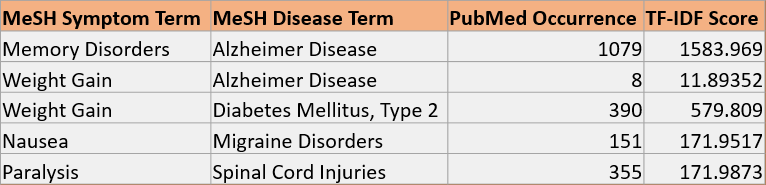
\includegraphics[width=\linewidth]{hsdnsymptdis}
		\caption{\footnotesize  Five records from a HSDN dataset mapping 147,978 symptom-disease relationships to their corresponding PubMed occurence frequencies and TF-IDF values. As you can see with AD, one MeSH disease term can link to multiple symptoms.}
		\label{hsdnsymptdis}
	\end{table}  
	
	A Java program was used to make E-utilities calls and obtain 7,109,429 PubMed records including one or more disease or symptom identified by 2011 MeSH descriptors in their MeSH metadata field.  These records contained 4,442 unique MeSH disease terms and 322 symptom descriptors, which represented 98.5\% of all diseases and 95.0\% of all symptoms in the 2011 MeSH vocabulary~\cite{hsdn}.  849,103 of these records contained at least one disease and one symptom term in their MeSH metadata.  The 147,978 symptom-disease relationships discovered were extracted into a dataset (Table~\ref{hsdnsymptdis}) linking MeSH symptom terms to disease terms by PubMed co-occurrence frequency and a common text mining measure known as the term frequency-inverse document frequency (TF-IDF) ~\cite{tfidf},~\cite{hsdn}.
	
	
	To determine TF-IDF values, each disease $j$ is identified by a vector of symptoms $d\textsubscript{j}$:
	\begin{equation}
	\label{dij}
	d\textsubscript{j} = (w\textsubscript{1,j}, w\textsubscript{2,j},... , w\textsubscript{n,j})
	\end{equation}
	
	\noindent where $w\textsubscript{i,j}$ is a measure of association strength between symptom $i$ and disease $j$.
	To account for publication biases and symptoms and diseases tending to appear more than others, the absolute co-occurrence $W\textsubscript{i,j}$ between a symptom $i$ and disease $j$, is used to calculate, and then substituted with, the TF-IDF $w\textsubscript{i,j}$:
	\begin{equation}
	 \label{wij}
	 w\textsubscript{i,j} = W\textsubscript{i,j}log\frac{N}{n\textsubscript{i}}
	 \end{equation}
	
	\noindent where $N$ is the dataset's total number of diseases and $n\textsubscript{i}$ is the number of diseases containing symptom $i$ ~\cite{tfidf},~\cite{hsdn}.  In general, the TF-IDF value provides a more representative frequency heuristic than absolute occurrence. 
	\begin{table}[h]
		\centering
		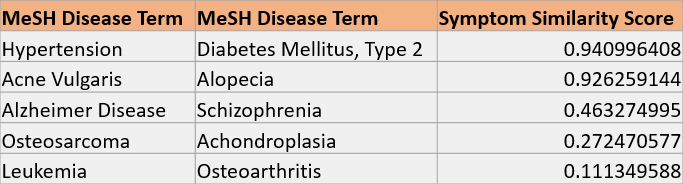
\includegraphics[width=\linewidth]{hsdndisdis}
		\caption{\footnotesize  Five records from a HSDN dataset mapping cosine similarities of symptom vectors for two MeSH disease terms to their respective pairings.  A total of 1,596 distinct diseases form 133,106 disease-disease connections in this dataset.}
		\label{hsdndisdis}
	\end{table}
	
	Another HSDN dataset (Table~\ref{hsdndisdis}) links similarity scores to 133,106 disease to disease connections, which include 1,596 unique MeSH disease terms.  The cosine similarity between diseases' symptom vectors is used as a similarity score.  The following equation is used to calculate the similarity between symptom vectors $d\textsubscript{x}$ and $d\textsubscript{y}$ for diseases $x$ and $y$:
		\begin{equation}
		\label{cosine}
		 cos(d_{x},d_{y}) = \frac{\sum_{i}d\textsubscript{x,i}d\textsubscript{y,i}}{\sqrt{\sum_{i}d_{x,i}^{2}}\sqrt{\sum_{i}d_{y,i}^{2}}}
		\end{equation}
	\noindent Cosine similarity will always range from 0 (no shared symptoms) to 1 (identical symptoms)~\cite{hsdn}.
	
	Given their extensive coverage and similarity equation validity, the HSDN's datasets (Table~\ref{hsdnsymptdis} and Table~\ref{hsdndisdis}) can be used as automated drug repurposing model development tools. 
	
	\subsection{Linux Shell Scripts}
	Linux is a UNIX-like operating system that uses the Bourne-Again SHell (Bash) programming language as its shell, a program that takes user commands from the keyboard and relays them to an operating system for execution"~\cite{shell}.  The command line is powerful and can serve many different functions.  Shell script files contain lists of commands that run in sequence\textemdash as if typed into the command line.  When script files are executed, the shell reads all commands and executes them in succession.  Scripts, which essentially automate command line tasks, could be helpful in automating drug repurposing as well.
	
	\section{A Working Prototype}
	\subsection{Interconnected Shell Scripts}
	We wrote two Linux shell scripts to consecutively execute multiple commands given one single command line call and simple user input. The first script, which quickly runs from the home directory, redirects to another directory where a script controlling the automated repurposing prototype executes.
	\begin{figure}[h]
		\centering
		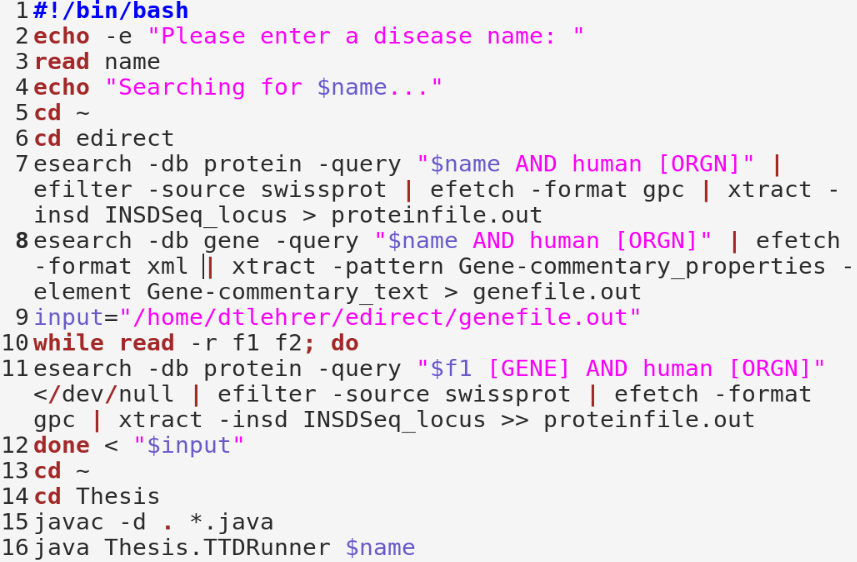
\includegraphics[width=\linewidth]{newscript}
		\caption{\footnotesize Verbatim code for the second of two Linux shell scripts.  This script asks the user for a disease name as input, retrieves that input, and uses EDirect queries to search the NCBI Protein and Gene databases for that particular disease.  UniProt IDs for disease-related proteins are then printed to one output file, while disease-related gene symbols are printed to another.  Each gene symbol is used to query the Protein database and output more disease-related proteins to \textit{proteinfile.out}, which is used in compilation and execution of an automated drug repurposing Java program, TTDRunner.}
		\label{linuxscript}
	\end{figure}
	\subsection{User Input}
	The Linux shell script seen in Figure~\ref{linuxscript} prompts the user to provide a disease name as input. It allows any input to be passed to a query, preserving the possibility of automated drug repurposing for many different diseases.
	\subsection{Obtaining Disease Data}
	Up-to-date disease, drug, and protein target data must be obtained for effective completion of the automated drug repurposing Java program.  Information downloaded from three TTD datasets and one HSDN dataset is used to form the basis of more expansive data cumulation in this program.  Full TTD datasets for protein targets with therapeutic potential, target to indication connections, and drug-indication relationships\textemdash similar to the samplings in Tables~\ref{ttduniprotall}, ~\ref{ttdtargetdisease}, and ~\ref{ttddrugdisease}, respectively\textemdash were downloaded along with a HSDN dataset linking disease name pairs to symptom similarity scores \cite{hsdn}.
	\subsection{Data Preprocessing}
	After obtaining disease data, datasets are merged and formatted for subsequent manipulation by a Java program.  The original TTD and HSDN datasets are downloaded as tab-delimited text files with one record per line.  We were able to open each of these files in Microsoft Excel, which sped up necessary preprocessing and allowed for simple conversion into easily parsable comma separated values (CSV) files.  
	
	The first TTD dataset contained 2,130 records similar to those in Table~\ref{ttduniprotall}.  To focus on the most reliable information, discontinued and research targets were pruned, leaving behind 904 (473 successful and 431 clinical trial) protein targets at the latest stages of testing.  The 904 remaining records were joined by TTD Target IDs with a set of 4,208 records similar to those in Table~\ref{ttddrugdisease}, where protein targets are linked to one or more indications.  The result of this merger was a new dataset containing 3,389 records with indication and protein target attributes.  The resulting records were joined by ICD codes with a set of 32,591 records formatted like those in Table~\ref{ttddrugdisease}, where existing drug projects are mapped to indications and their ICD codes.  This combination added two attributes (TTD Drug IDs and Drug Names) to each of the 3,389 records to form the completely merged TTD dataset.  In most cases, more than one drug project was linked to target-indication combinations.
	
	The HSDN dataset sampled in Table~\ref{hsdndisdis} contains 133,306 disease to disease connections amongst 1,596 distinct diseases \cite{hsdn}.  This means most of the dataset's diseases are compared to several other diseases via cosine similarity scores.  Having two MeSH disease term attributes complicates data retrieval, however, so the dataset was reorganized to include 1,596 records linking disease terms to indexed lists of connected diseases and similarity scores.  All disease occurrences could be valuable, so further preprocessing was not performed.
	
   
	\subsection{Protein Data Extraction}
	As seen in Figure~\ref{linuxscript}, script-supplied disease name input is passed to an EDirect query that searches the Protein database\textemdash specifically the UniProtKB/Swiss-Prot source\textemdash for input-related human proteins.  This query's output is formatted in a way that allows for automated metadata extraction of the proteins' UniProt IDs, which are written, one per line, to a text file used in the Java program.
	\subsection{Data Integration}
	Using extracted and preprocessed data, the Java program stores records as ArrayLists of Strings.  If a merged TTD dataset record's UniProt ID matches any of the input-related target proteins' UniProt IDs, the record is saved for further filtration and analysis.  Data retrieved from these saved records is used to create lists of disease-related proteins, potential protein targets, and potential drugs for repurposing.  Of the records with input-related UniProt IDs, protein data is mapped to drugs and indications.  This mapping, illustrated in Figure~\ref{prototypestructure} allows drug projects to be weighted based on EDirect query results from within the Java program.
		\begin{figure}[h]
			\centering
			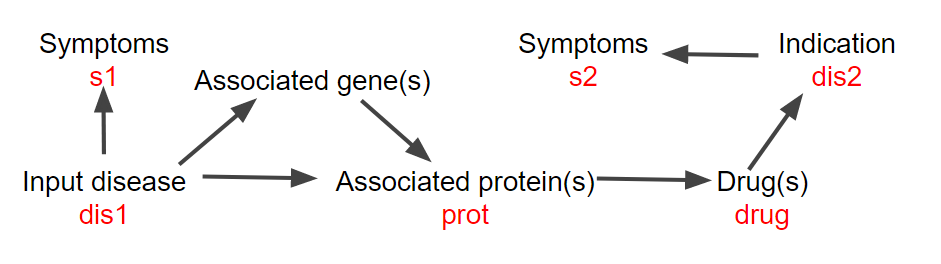
\includegraphics[width=\linewidth]{prototypestructure}
			\caption{\footnotesize General prototype structure, showing integrated data field relationships.  Starting from input diseases, we can derive valuable disease-related symptom, gene, and protein data.  Disease-related proteins may be targeted by one or more drugs to treat corresponding indications, which have their own set of symptoms.}
			\label{prototypestructure}
		\end{figure}
	\subsection{Weighting Pre-Approved Drugs For Treatment} \label{weights}
	After filtering records and querying the Entrez databases, the Java program prepares a set of potential pre-approved drugs for treatment.  These pre-approved drugs for treatment could be provided to the user as is, but the number of drugs depends on the disease queried\textemdash and diseases with many biomedical literature citations (e.g., diabetes) will often return several thousands of potential therapeutic drugs.  To simplify and differentiate drug output, a series of three weights is computed for each of the potential drug projects:
	\begin{enumerate}
		\item \textbf{Input Disease to Target Protein ($w_1$):}  relates the number of PubMed abstracts containing both the target protein (prot) and input disease name (dis1) $A_{pd}$ to the number of abstract results containing the input disease name $A_{d}$.
		\begin{equation}
		\label{weight1}
		w\textsubscript{1} = \frac{A_{pd}}{A_{d}} 
		\end{equation}
		\item \textbf{Input Disease to Drug Indication ($w_2$):} relates the number of PubMed abstracts containing both the drug indication name (ind) and input disease name (dis1) $A_{id}$ to the number of abstract results containing the input disease name $A_{d}$.
		\begin{equation}
		\label{weight2}
		w\textsubscript{2} = \frac{A_{id}}{A_{d}} 
		\end{equation}
		\item \textbf{Input Disease Symptoms to Indication Symptoms ($w_3$):} obtained from a preprocessed version of the HSDN dataset sampled in Table~\ref{hsdndisdis}\textemdash equal to the cosine similarity between symptom vectors $d\textsubscript{x}$ and $d\textsubscript{y}$ for input disease $x$ (dis1) and drug indication $y$ (dis2).  See Equation (\ref{cosine}) for more information.
	\end{enumerate}  
	\begin{equation}
	\label{weight3}
	w\textsubscript{3} = cos(d_{x},d_{y})
	\end{equation}
	
	All three weights ($w_{1}$, $w_{2}$, and $w_{3}$) should range from 0 to 1.  The first two weights ($w_{1}$ and $w_{2}$) are calculated from EDirect query result counts.  In both cases, the numerator ($A_{pd}$ and $A_{id}$) should be a subset of the denominator ($A_{d}$), because another parameter is added to the esearch query in the numerator\textemdash further restricting the result set.  We know that $w_{3}$ will range from 0 to 1 due to the nature of cosine similarity \cite{hsdn}.  
	
	In all three cases, higher weights should be favored and indicate greater repurposing potential for their respective drug.  With this rule in mind, and a goal of easier indication of drugs with the highest repurposing potentials for a given disease, a combined weight $W_{c}$ is calculated for each drug:
	\begin{equation}
	\label{combinedweight}
	W\textsubscript{c} = 0.15w_{1} + 0.5w_{2} + 0.35w_{3}
	\end{equation}
	The smallest coefficient (0.15) is attributed to the input disease to target protein weight, $w_{1}$, because this weight is relatively undifferentiated given how many drugs share the same target proteins.  At 0.35 or 35\%, the input disease symptoms to indication symptoms weight is multiplied more than $w_{1}$, but less than $w_{3}$.  It provides some meaningful information, but many symptoms apply to a wide range of diseases, and these correlations alone do not always imply similar drug effectiveness.  The largest multiplier (0.5) is assigned to the input disease to drug indication weight, $w_{2}$, due to higher probability that drugs and diseases mentioned in the same PubMed abstracts are related in some meaningful way.  Beyond this reasoning, each weight's applied coefficients are relatively arbitrary at this point.  With further program testing and model training, Equation~(\ref{combinedweight}) will likely be adjusted to provide more accurate results.
	
	\section{Experimental Results}
	Completion of our automated drug repurposing prototype for AD suggests 14,852 pre-approved drugs for potential AD treatment.  These drugs target 203 unique proteins, a subset of 532 AD-related proteins obtained from Protein and Gene database EDirect queries.  Mentioned in Section~\ref{omics}, Zhang et al.~\cite{zhang16} suggested 92 existing drugs for potential AD treatment repurposing, and 70 of these 92 drugs (76\% overlap) were identified via automation. Though much smaller than our prototype's drug suggestion set, Zhang et al.~\cite{zhang16} identified a similar amount of AD-related proteins (524) through manual data extraction, but only 8 potential protein targets for anti-AD drug development.  
	
	Because many drugs share target proteins and/or indications, they also have similar weights. We assigned weight rankings to each of the three calculated weight categories, ranking the the highest weight(s) in each category as 1, the next highest as 2, and so on. Equal weights share the same rank, but ranks are not skipped due to ties.  For example, drug weights of 1.0, 1.0, 0.5, and 0.7 would be ranked 1, 1, 3, and 2, respectively.  Using this ranking system, 252 unique ranks were assigned for input to drug indication weights, while target protein weights received 55 ranks, and symptom weights only had 30 differentiated weights.  
	
			\begin{figure}[h]
				\centering
				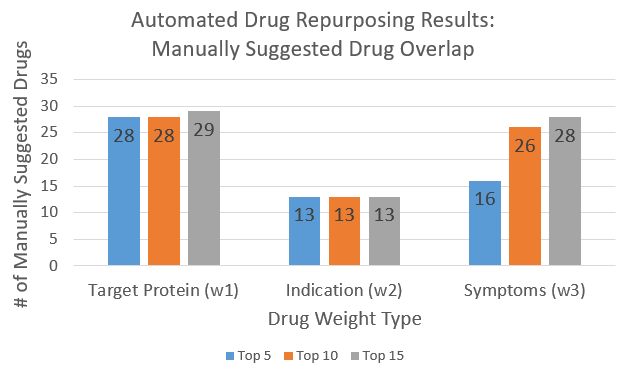
\includegraphics[width=\linewidth]{weightsfig}
				\caption{\footnotesize Black box structure of our automated drug repurposing program that takes a disease name as input and outputs top potential pre-approved drugs for repurposing through internal data mining algorithms.}
				\label{weightsfig}
			\end{figure} 
	
	\noindent As seen in Figure~\ref{weightsfig}, we gathered the number of manually suggested drugs in the top 5, 10, and 15 ranks for each of our three drug weights.  The target protein weight had more drugs in all three weight rank categories, followed by the symptom weight, and then the indication weight.  This could be attributed to drug indication weights being more differentiated and having more ranks.
	
	Closer individual drug weight analysis reveals 13 of the 70 suggested drugs have an input disease to drug indication weight of 1, meaning EDirect queries for input disease and indication return the same amount of results as queries with only input disease names, and the drugs are already indicated for AD treatment.  Likewise, these same drugs have symptom weights of 1.  For improved comparison, and to better replicate manual AD drug repurposing findings~\cite{zhang16}, we need to preserve drug overlap while filtering out less meaningful drugs.  Additional drug information may be helpful in shrinking our suggested drug set to more manageable standards.
	\section{Future Work: Automated Opportunities}
		\begin{figure}[h]
			\centering
			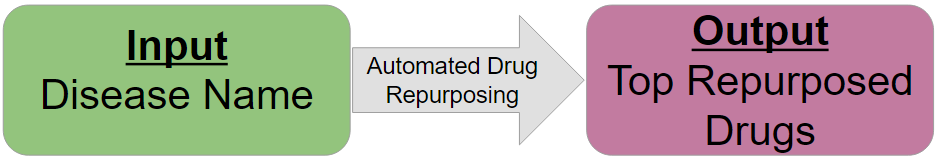
\includegraphics[width=\linewidth]{autorepurp}
			\caption{\footnotesize Automated drug repurposing comparison to manual drug repurposing results for Alzheimer's disease~\cite{zhang16}.  Each drug is weighted three different ways, each individual weight is ranked, and drugs appearing within certain ranking sections for both automated and manual drug repurposing are recorded.}
			\label{autorepurp}
		\end{figure} 
		
		By identifying tools for automated drug repurposing and using databases such as PubMed and TTD, we have developed an automated drug repurposing working prototype, which has streamlined the process of biomedical data retrieval, analysis, and manipulation for drug repurposing.  The program outputs a list of drugs suggested for repurposing, each with three individualized weights, as desired.  Without more extensive comparison to manual drug repurposing results and further program result validation and analysis, however, a conclusion cannot be made on the effectiveness of this automated drug repurposing prototype.
		
		There is no evidence of a fully effective and validated automated drug repurposing program similar to the one depicted in Figure~\ref{autorepurp}, however, we expect continued research and collaboration to produce something comparable.  Additionally, drug discovery can be automated beyond drug repurposing.  Automation of one small part of the FDA's lengthy, seven-step drug development process~\cite{xu} could drastically reduce drug discovery time.  Given the process's current length, many steps can be shortened\textemdash and they all present great opportunities for more efficient drug discovery.   
		
		Discussed in Section~\ref{standardized}, researchers already use automation in lead identification, when compiled biological material libraries are screened directly against drug targets for activity. For this reason, we predict automation will carry over into more drug discovery steps as technology advances.  
	
	\section{Conclusion}
	By analyzing the evolving method of drug repurposing based on omics data mining, recognizing the opportunity for growth beyond manual data extraction, and identifying tools for automated drug repurposing, We have developed an automated drug repurposing framework and working prototype.  Integration of Linux shell scripts, EDirect, and the Java programming language has streamlined the process of biomedical data retrieval, analysis, and manipulation for the purposes of drug repurposing.  Program output is formatted as desired, and a subset of initial drugs is suggested for repurposing potential.  Without further program result validation and analysis, however, a conclusion cannot be made on the effectiveness of this automated drug repurposing prototype.  Moving forward, we will continue to compare prototype output to the manual results of Zhang et al. in their studies on diabetes~\cite{zhang15} and AD~\cite{zhang16}, as similar drug suggestions would provide a degree of validation to this system.  Java algorithm and weighting equation fine-tuning will likely follow. A functioning program is promising, but we need better results to suggest true long-term program value.  With further research, additional data sources, and complete drug suggestion filtering, we could improve prototype results and transition to a better working model.
	
	Accounting for drug discovery's recent trends and theoretical limitations, we predict that automated drug discovery approaches, such as automated drug repurposing, will grow and become commonplace, evolving medicine's landscape.  As technological data continues to grow with biomedical data stores, opportunities to improve costly inefficiencies will likely fuel development of well-recognized and respected automated drug discovery programs. These programs will take disease names as input and output repurposed drugs for treatment.  With existing drug repurposing method refinement, and automated algorithm fine-tuning, utilizing vast amounts of biomedical data will reduce waste and make drug discovery more efficient. As automated drug discovery processes grow and become more consistently effective in the near future of a world filled with automation, completely automated drug development may emerge sooner than expected.  

% This line is used to build the bibliography.  In this case, we use the 
% \bibliography command to include the file sample.bib, which contains our
% bibtex database.  The bibtex command (which our Latex IDE runs for us) processes
% our Latex document and scans our Bibtex file for matching citations, and then
% generates the bibligraphy based on the style selection we made at the top
% of the document.

\bibliography{Lehrer_SOTF}

%\clearpage
%\newpage
\appendix
\subsection{Reflection}
My undergraduate career at the College of Saint Benedict and Saint John's University (CSB/SJU) has fittingly culminated with CS373 research and state-of-the-field (SOTF) work.  By combining interests in computer science (CS) and medicine, my chosen research path integrated learned concepts from previous coursework, while still allowing me to explore new topics and make interesting discoveries.  

As a computer science major and pre-medicine student at CSB/SJU, my previous coursework provided a foundation for success on this project.  Beginning with first-year seminar (FYS), my writing skills developed through research projects and other exercises, making me more confident in constructing lengthy papers and searching scientific literature sources.  I also received my first exposure to CS during my first semester at CSB/SJU.  As an undecided major, I felt inclined to major in CS when I discovered computing's possibilities and found myself completing CS homework before other assignments. 

Foundational programming skills taught in early CS courses undoubtedly assisted me in this project.  Learning programming languages like Jython and Java allowed me to structure more coherent algorithms, and provided confidence to explore other programming languages.  Specifically, Linux command line exercises and Java programming assignments developed backgrounds for self-teaching and personal growth. I used both tools extensively in prototype program development, but needed to research new techniques and grow these skills at standstills. Database and data mining courses also closely benefited my research work.  Data mining interests directed my initial research exploration, while database knowledge was useful when working with sources such as PubMed and TTD.  Beginning this research, biology and chemistry backgrounds helped me understand basic terms and concepts in dense research articles, but my CS department summer research opportunity familiarized me with research methods and techniques that enabled more complete textual understanding.  Weekly meetings with  Dr. Rahal helped guide the direction of my research and provided me with new ideas.  I was fortunate to have that extra research experience before enrolling in CS373.

CS373 and this project's challenges made me a more well-rounded computer scientist.  I will always remember our class motto ("enough words, no more"), more engaging presentation techniques, and the importance of consistent self-learning.  By practicing these skills, they have become habits that will help me in the future.  I am truly grateful for this profound learning experience and all who made it possible. 

\end{document}
